\chapter{Nash Equilibria}
\label{chapter:Nash}
%\documentclass[10pt]{article}
%\begin{document}

%%%%%%%%%%%%%%%%%%%%%%%%%%%%%%%%%%%%%%%%%%%%%%%%%%%%%%%%%%
%%%%%			Introduction Chapter 1				%%%%%%
%%%%%												%%%%%%
%%%%%												%%%%%%
%%%%%%%%%%%%%%%%%%%%%%%%%%%%%%%%%%%%%%%%%%%%%%%%%%%%%%%%%%

\section{Nash Equilibria}
-- rechtstreeks uit FlipIt paper --\\
As a second step, we are interested in finding Nash equilibria, points
for which neither player will increase his benefit by changing his rate of play. More
formally, a Nash equilibrium for the periodic game is a point $(\alpha_{0}^{*},\alpha_{1}^{*})$ such that
the defender's benefit $\beta_{0}(\alpha_{0},\alpha_{1}^{*}) $is maximized at $\alpha_{0}= \alpha_{0}^{*}$ and the attacker's benefit
$\beta_{1}(\alpha_{0}^{*},\alpha_{1}) $ is maximized at $\alpha_{1}= \alpha_{1}^{*}$ .
To begin with, some useful notation. We denote by opt0($\alpha_{1}$) the set of values (rates
of play $\alpha_{0}$) that optimize the benefit of the defender for a fixed rate of play $\alpha_{1}$ of the
attacker. Similarly, we denote by opt1($\alpha_{0}$) the set of values (rates of play $\alpha_{1}$) that optimize
the benefit of the attacker for a fixed rate of play $\alpha_{0}$ of the defender. The following
theorem specifies Nash equilibria for the periodic game and is proven in Appendix A. \\
\begin{figure}[hbtp]
\caption{This figure shows the three subcategories of each case. 'A' stands for Case 2.A: $\delta_{D} \geq d+\delta_{A} \geq \delta_{A}$ and 'B' stands for Case 2.B: $d+\delta_{A} \geq \delta_{D} \geq  \delta_{A} $ }
\centering
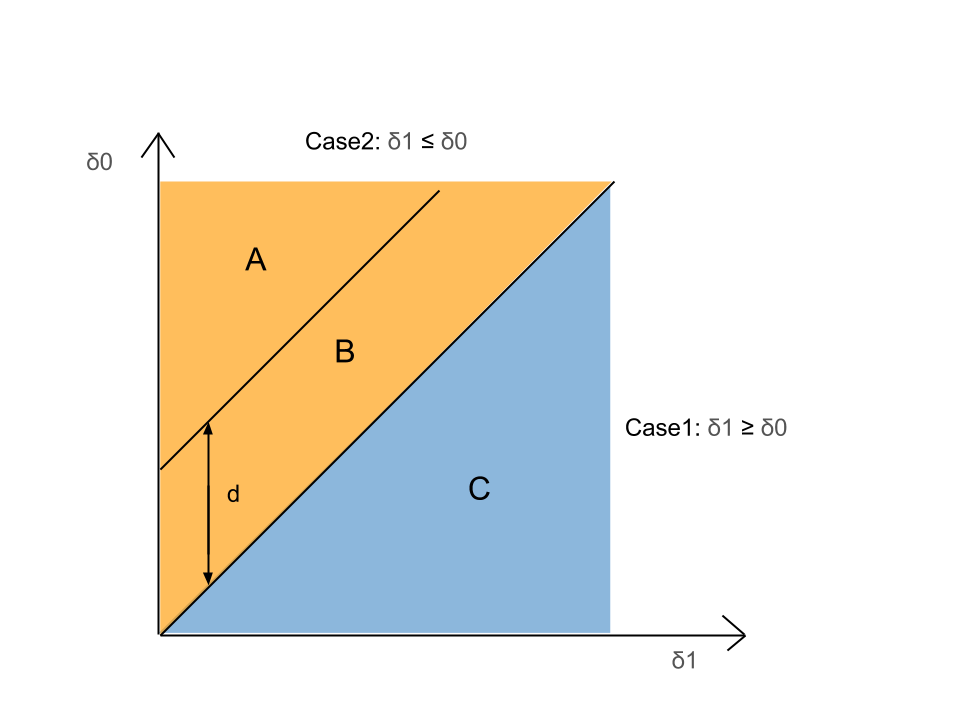
\includegraphics[scale=0.4]{Images/bestresp.png}
\label{grafiekbestr}
\end{figure}

\subsection{Determining the piecewise functions $opt_{D}(\delta_{A})$}

Nash equilibria are points with the property that neither player benefits by deviating in isolation form equilibrium. We can compute Nash Equilibria for the periodic game as an intersection points of curvest opt0 and opt1. To determine opt0(a0) we need to compute the derivative of  $\beta_{0}(\alpha_{0},\alpha_{1}) $ for a fixed $\alpha_{1}$. We consider two cases:\\

\subsection*{Case 1: $\delta_{D} \leq \delta_{A} $}
The benefit formula obtained previously for this case is as follows:
\begin{equation*}
\beta_{D}(\alpha_{D},\alpha_{A}) = 1 - \dfrac{\delta_{D}}{2\delta_{A}} - \dfrac{k_{D}}{\delta_{D}} - \dfrac{d^{2}}{2\delta_{D}\delta_{A}} + \dfrac{d}{\delta_{A}}
\end{equation*}
If we take the partial derivative for a fixed $\delta_{1}$ we get the following result:
\begin{equation*}\label{formdelta}
\frac{\partial \beta_{D}(\alpha_{D},\alpha_{A})}{\partial \alpha_{D}} = - \dfrac{1}{2\delta_{A}} + \dfrac{k_{D}}{\delta_{D}^{2}} + \dfrac{d^{2}}{2\delta_{D}^{2}\delta_{A}}
\end{equation*}

The stationary points (maximum, minimum) can be found by setting the first derivative equal to zero and finding the roots of the resulting equation:
\begin{equation*}
\frac{\partial \beta_{D}(\alpha_{D},\alpha_{A})}{\partial \alpha_{D}} =0 ~~~~~~ =>~~~~~~ \delta_{D} = \sqrt{2\delta_{A}k_{D} + d^{2}}
\end{equation*}

This leads to the following deduction: The function increases on $[0, \sqrt{2\delta_{A}k_{D} + d^{2}}]$ and is decreasing on $[\sqrt{2\delta_{A}k_{D} + d^{2}}, \infty]$ So we got a maximum on $\delta_{D} = min \{ \delta_{A}, \sqrt{2\delta_{A}k_{D} + d^{2}} \} $. The minimum of the two values is needed because $\delta_{D}$ cannot be bigger than $\delta_{A}$. \\
~~\\


\subsection*{Case 2.A: $\delta_{D} \geq d+\delta_{A} \geq \delta_{A} $ }

The benefit formula obtained previously for this case is as follows:
\begin{equation*}
\dfrac{t \beta_{D}(\alpha_{D},\alpha_{A})}{\partial \alpha_{D}} = \dfrac{\delta_{A}}{2\delta_{D}} + \dfrac{d}{\delta_{D}} - \dfrac{k_{D}}{\delta_{D}}
\end{equation*}

The derivative of the above formula for a fixed $\delta_{A}$ results in the following:
\begin{equation*}
\frac{\partial \beta_{D}(\alpha_{D},\alpha_{A})}{\partial \alpha_{D}} = -\dfrac{\delta_{A}}{2\delta_{D}^{2}} - \dfrac{d}{\delta_{D}^{2}} + \dfrac{k_{D}}{\delta_{D}^{2}}
\end{equation*}
The obtain the stationary points the first derivative is set equal to zero and the roots of the resulting equation are found:
\begin{equation*}
\frac{\partial \beta_{D}(\alpha_{D},\alpha_{A})}{\partial \alpha_{D}} =0 ~~~~~~ =>~~~~~~ \delta_{A} = 2(k_{D}-d) = dk_{D} - 2d
\end{equation*}

This leads to the following deduction:
\begin{description}
\item If $k_{D} \leq d$ 
\begin{description}
\item decreasing $ \delta_{A} < 2(k_{D} -d)$
\item increasing  $\delta_{A} > 2(k_{D} -d)$ 
\end{description}
\item If $k_{D} > d$ 
\begin{description}
\item increasing $ \delta_{A} < 2(k_{D} -d)$
\item decreasing  $\delta_{A} > 2(k_{D} -d)$ 
\end{description}
\end{description}
~~\\

\subsection*{Case 2.B: $d+\delta_{A} \geq \delta_{D} \geq  \delta_{A} $} 

The benefit formula obtained previously for this case is as follows:
\begin{equation*}
\dfrac{\beta_{D}(\alpha_{D},\alpha_{A})}{\partial \alpha_{D}} = \dfrac{\delta_{A}}{2\delta_{D}} + \dfrac{d}{\delta_{D}} - \dfrac{k_{D}}{\delta_{D}} - \dfrac{(d-(\delta_{D} - \delta_{A}))^{2}}{d\delta_{D}\delta_{A}}
\end{equation*}

The derivative of the above formula for a fixed $\delta_{A}$ results in the following:
\begin{equation*}
\frac{\partial \beta_{D}(\alpha_{D},\alpha_{A})}{\partial \alpha_{D}} =  - \dfrac{1}{2\delta_{D}} + \dfrac{k_{D}}{\delta_{D}^{2}} + \dfrac{d^{2}}{2\delta_{D}^{2}\delta_{A}}
\end{equation*}


The stationary points (maximum, minimum) can be found by setting the first derivative equal to zero and finding the roots of the resulting equation:

\begin{equation*}
\frac{\partial \beta_{D}(\alpha_{D},\alpha_{A})}{\partial \alpha_{D}} =0 ~~~~~~ =>~~~~~~ \delta_{D} = \sqrt{2\delta_{A}k_{D} + d^{2}}
\end{equation*}


This leads to the following deduction: The function increases on $[0, \sqrt{2\delta_{A}k_{D} + d^{2}}]$ and is decreasing on $[\sqrt{2\delta_{A}k_{D} + d^{2}}, \infty]$ So we got a maximum on $\delta_{D} = minimum \{ \delta_{A}, \sqrt{2\delta_{A}k_{D} + d^{2}} \} $ \\

\subsubsection{Best responses}
The optimum functions will be piecewise functions. There will be different optimum functions depending on $k_{D}$ and $d$. We distinguish for these two cases, three sub cases for different values of $\delta_{A}$. 

\subsection*{$k_{D} \leq d$}
Because $k_{D} \leq d$, the term $2(k_{D} - d)$ will always be negative. We point out that $\delta_{A}$ and $\delta_{D}$ are positive rates. 
\begin{itemize}
\item if $\delta_{A} < 2(k_{D} - d)$ \\
This means that $\delta_{A}$ has to be negative which is not possible. For case the defender will not play.
\item $\delta_{A} = 2(k_{D} - d)$ \\
$\delta_{A}$ is negative or equal to 0 so the attacker will not play. For case 1 and case 2.b the defender will also not play.
\item $\delta_{A} > 2(k_{D} - d)$ \\
Case 2.a it is increasing for every value $\delta_{A} \in [0,\infty]$.  For case 1 together with case 2.b the optimal benefit is achieved at rate $\delta_{D} = \sqrt{d^{2} + 2\delta_{A}k_{D}}$.
\end{itemize}


\subsubsection{$k_{D} > d$}
Because $k_{D} > d$, the term $2(k_{D} - d)$ will always be positive. We point out that $\delta_{A}$ and $\delta_{D}$ are positive rates.
\begin{itemize}
\item if $\delta_{A} < 2(k_{D} - d)$ \\
From case 2.a it follows that the benefit of the defender increases. From case 1 and case 2.b together the optimal benefit of the defender is achieved at rate $\delta_{D} = \sqrt{d^{2} + 2\delta_{A}k_{D}}$.
\item $\delta_{A} = 2(k_{D} - d)$ \\
From case 2.a it follows that $\beta_{D}(\delta_{D},\delta_{A})=0$, for all $\delta_{A} \in [0,2(k_{D} - d)]$. From case 1 and case 2.b together the optimal benefit for the defender is achieved for all rates $\delta_{D} \in [0, \sqrt{d^{2} + 2\delta_{A}k_{D}}]$.
\item $\delta_{A} > 2(k_{D} - d)$ \\
For case 2.a the benefit is decreasing. From case 1 and case 2.b the best strategy for the defender is not playing at all. 
\end{itemize}
\todo{dat laatste nog eens nakijken}

From this analyses we can compute $opt_{D}(\delta_{A})$ for two different cases as:
 \begin{displaymath}
  opt_{D}(\delta_{A}) = \left\{
     \begin{array}{lr}
       0, & \delta_{A} < 2(k_{D} - d)\\
       0, & \delta_{A} = 2(k_{D} - d) \\
       \sqrt{d^{2} + 2\delta_{A}k_{D}}, & \delta_{A} > 2(k_{D} - d)
     \end{array}
   \right.
\end{displaymath}

For case :
 \begin{displaymath}
  opt_{D}(\delta_{A}) = \left\{
     \begin{array}{lr}
       \sqrt{d^{2} + 2\delta_{A}k_{D}}, & \delta_{A} < 2(k_{D} - d)\\
       \big[0,\sqrt{d^{2} + 2\delta_{A}k_{D}}\big], & \delta_{A} = 2(k_{D} - d) \\
       0, & \delta_{A} > 2(k_{D} - d)
     \end{array}
   \right.
\end{displaymath}


%*****************************************************************
%
% optimum functies voor beta A
%
%*********************************************************************
\subsection{Determining the piecewise functions $opt_{A}(\delta_{D})$}
We still consider the case where $d < \delta_{D}$. \\
To determine the Nash equilibria we also need to determine $opt_{A}(\delta_{D})$ by computing the derivative of $\beta_{A}(\delta_{D},\delta_{A})$ for a fixed $\delta_{D}$. We consider 2 cases: \\

\subsection*{Case 1: $\delta_{A} \geq \delta_{D}$}

The benefit formula obtained previously for this case is as follows:
\begin{equation*}
\beta_{A}(\delta_{D},\delta_{A}) =\dfrac{\delta_{D}}{2\delta_{A}} - \dfrac{k_{A}}{\delta_{A}} + \dfrac{d^{2}}{2\delta_{D}\delta_{A}^{2}} - \dfrac{d}{\delta_{A}}
\end{equation*}
The derivative for a fixed $\delta_{D}$ is as follows:
\begin{equation*}
\dfrac{\partial \beta_{A}(\delta_{D},\delta_{A})}{\partial \delta_{A}} = -\dfrac{\delta_{D}}{2\delta_{A}^{2}} + \dfrac{k_{A}}{\delta_{A}^{2}} - \dfrac{d^{2}}{2\delta_{D}\delta_{A}^{2}} + \dfrac{d}{\delta_{A}^{2}}
\end{equation*}
The stationary points (maximum, minimum) can be found by setting the first derivative equal to zero and finding the roots of the resulting equation:
\begin{equation*}
\frac{\partial \beta_{A}(\alpha_{D},\alpha_{A})}{\partial \alpha_{D}} =0 ~~~~~~ =>~~~~~~ 2k_{A} = \dfrac{(\delta_{D}-d)^{2}}{\delta_{D}}
\end{equation*}

It follows that $\beta_{A}(\delta_{D},\cdot)$ is increasing if $2k_{A} < (\delta_{D} - d)^{2} / \delta_{D}$ and decreasing if $2k_{A} > (\delta_{D} - d)^{2} / \delta_{D}$. \\

\subsection*{Case 2.A: $\delta_{D} \geq d+\delta_{A} \geq \delta_{A} $ }
The benefit formula obtained previously for this case is as follows:
\begin{equation*}
\beta_{A}(\delta_{D},\delta_{A}) =1- \dfrac{\delta_{A}}{2\delta_{D}} - \dfrac{k_{A}}{\delta_{A}} - \dfrac{d}{\delta_{D}}
\end{equation*}
The derivative for a fixed $\delta_{D}$ is as follows:
\begin{equation*}
\dfrac{\partial \beta_{A}(\delta_{D},\delta_{A})}{\partial \delta_{A}} = \dfrac{-1}{2\delta_{D}} + \dfrac{k_{A}}{\delta_{A}^{2}}
\end{equation*}
The stationary points (maximum, minimum) can be found by setting the first derivative equal to zero and finding the roots of the resulting equation:
\begin{equation*}
\frac{\partial \beta_{A}(\alpha_{D},\alpha_{A})}{\partial \alpha_{D}} =0 ~~~~~~ =>~~~~~~ \delta_{A} = \sqrt{2\delta_{D}k_{A}}
\end{equation*}
it follows that $\beta_{A}(\delta_{D},\cdot)$ is increasing on $[0,\sqrt{2k_{A}\delta_{D}}]$ and decreasing on $[\sqrt{2k_{A}\delta_{D}}, \infty]$ and thus has a maximum on $\delta_{A} = maximum \{\delta_{D}, \sqrt{2k_{A}\delta_{D}} \} $. The maximum between $\delta_{D}$ and $ \sqrt{2k_{A}\delta_{D}}$ is needed because $\delta_{A} $ cannot exceed $\delta_{D}$ in this case. \\

\subsection*{Case 2.B: $d+\delta_{A} \geq \delta_{D} \geq  \delta_{A} $} 

The benefit formula obtained previously for this case is as follows: 
\begin{equation*}
\beta_{A}(\delta_{D},\delta_{A}) = 1 - \dfrac{\delta_{A}}{2\delta_{D}} - \dfrac{d}{\delta_{A}} - \dfrac{k_{A}}{\delta_{A}} + \dfrac{(d-(\delta_{D}-\delta_{A})^{2}}{2\delta_{D}\delta_{A}} 
\end{equation*}
The derivative for a fixed $\delta_{D}$ is as follows:
\begin{equation*}
\dfrac{\partial \beta_{A}(\delta_{D},\delta_{A})}{\partial \delta_{A}} = -\dfrac{\delta_{D}}{2\delta_{A}^{2}} + \dfrac{k_{A}}{\delta_{A}^{2}} - \dfrac{d^{2}}{2\delta_{D}\delta_{A}^{2}} + \dfrac{d}{\delta_{A}^{2}}
\end{equation*}
The stationary points (maximum, minimum) can be found by setting the first derivative equal to zero and finding the roots of the resulting equation:
\begin{equation*}
\frac{\partial \beta_{A}(\alpha_{D},\alpha_{A})}{\partial \alpha_{D}} =0 ~~~~~~ =>~~~~~~ 2k_{A} = \dfrac{(\delta_{D}-d)^{2}}{\delta_{D}}
\end{equation*}

it follows that $\beta_{A}(\delta_{D},\cdot)$ is increasing if $2k_{A} < (\delta_{D} - d)^{2} / \delta_{D}$ and decreasing if $2k_{A} > (\delta_{D} - d)^{2} / \delta_{D}$. This is the same result as in case 1.\\


\subsubsection{Best responses}
The optimum functions will be piecewise functions. We distinguish three cases for different values of $\delta_{d}$ and $k_{A}$. 


For this term $\dfrac{(\delta_{D}-d)^{2}}{\delta_{D}} $ , $d$ has to be bigger than  $\delta_{D}$ because the cost $k_{A}$ cannot be negative. This was an assumption that was already made, because the benefit of the defender will always be 1 if $d$ is bigger than  $\delta_{D}$.
\begin{itemize}
\item if $2k_{A} < \dfrac{(\delta_{D}-d)^{2}}{\delta_{D}} $ \\
Then for case 1 and case 2.b the benefit of the defender is increasing. From case 2.a follows that the optimal benefit for the attacker is achieved at the rate $\delta_{A} = \delta_{D}$
\item if $2k_{A} = \dfrac{(\delta_{D}-d)^{2}}{\delta_{D}} $ \\
From case 1 and case 2.b it follows that $\beta_{D}(\delta_{D},\delta_{A})=0$, for all $\delta_{A} \in [0,\dfrac{(\delta_{D}-d)^{2}}{2k_{A}})]$. From case 2.a the optimal benefit for the defender is achieved for all rates $\delta_{A} \in [0, \delta_{D}]$.
\item if $2k_{A} > \dfrac{(\delta_{D}-d)^{2}}{\delta_{D}} $ \\
All decreasing.
\end{itemize}

This brings us to the following opt function for : \todo{juiste resultaten hier nog invullen}
From this analyses we can compute $opt_{D}(\delta_{A})$ for two different cases as:
 \begin{displaymath}
  opt_{D}(\delta_{A}) = \left\{
     \begin{array}{lr}
       0, & \delta_{A} < 2(k_{D} - d)\\
       0, & \delta_{A} = 2(k_{D} - d) \\
       \sqrt{d^{2} + 2\delta_{A}k_{D}}, & \delta_{A} > 2(k_{D} - d)
     \end{array}
   \right.
\end{displaymath}

\todo{ kA met kD vergelijken en nash evenwichten vinden}
\todo{ een voorbeeld invullen met specifieke waarden}